% !TEX root = ../OT4ML.tex

%%%%%%%%%%%%%%%%%%%%%%%%%%%%%%%%%%%%%%%%%%%%%%%%%%%%%%%%%%%%%%%%%%%%%%%%%%%
%%%%%%%%%%%%%%%%%%%%%%%%%%%%%%%%%%%%%%%%%%%%%%%%%%%%%%%%%%%%%%%%%%%%%%%%%%%
%%%%%%%%%%%%%%%%%%%%%%%%%%%%%%%%%%%%%%%%%%%%%%%%%%%%%%%%%%%%%%%%%%%%%%%%%%%
\chapter{Optimal Matching between Point Clouds}
\index{matching!optimal}% strictindex
\label{sec-matching}

This opening chapter isolates the simplest form of optimal transport: pairing two finite, equally weighted point clouds of the same cardinality. The stakes are algorithmic and geometric at once: one sees the combinatorial nature of transport, the special simplicity of the line, and the limitations of permutations once cardinalities or weights differ. Classical assignment algorithms such as the Hungarian and auction methods~\cite{Kuhn1955,bertsekas1992auction} provide the computational backdrop, while the weighted examples motivate the Kantorovich relaxation.
\index{Hungarian primal-dual method}% strictindex
\index{Kantorovich!relaxation}% strictindex

%%%%%%%%%%%%%%%%%%%%%%%%%%%%%%%%%%%%%%%%%%%%%%%%%%%%%%%%%%%%%%%%%%%%%%%%%%%
\section{Monge Problem for Discrete Points}
\index{Monge!problem}% strictindex
\label{sec-monge-pbm}

This section formulates matching as Monge's deterministic transport problem on two equally weighted clouds. The one-dimensional case is a transparent reference case where the optimal map can be read off by sorting.

%%%%%%%
\paragraph{Assignment problem.}
\index{assignment problem}% strictindex

Let $\C\in\RR^{n\times n}$ be a cost matrix, where $\C_{i,j}$ is the cost of pairing source $i$ with target $j$, and let $\Perm(n)$ denote the set of bijections of $\range{n}=\{1,\ldots,n\}$. The optimal assignment problem is
\index{cost!matrix}% strictindex
\eql{\label{eq-optimal-assignment}
	\umin{\sigma \in \Perm(n)} \frac{1}{n}\sum_{i=1}^n \C_{i,\sigma(i)}.
}
When $\C_{i,j}=c(x_i,y_j)$, this is the Monge problem between the empirical measures $n^{-1}\sum_i\delta_{x_i}$ and $n^{-1}\sum_j\delta_{y_j}$. The normalization by $1/n$ records the mass of each atom but does not change the minimizing permutation. Exhaustive search evaluates all $n!$ permutations and is therefore impractical; efficient methods exploit geometry or linear-programming duality. Unless additional assumptions are imposed on $\C$, the optimizer need not be unique.

\paragraph{Convex costs on the line.}

On the line, convexity turns the order of the points into a complete optimality certificate.

\begin{proposition}[Monotone matching on the line]\label{prop-matching-1d-monotone}
\index{monotone!matching}% strictindex
Assume that $x_1,\ldots,x_n$ are pairwise distinct and that $y_1,\ldots,y_n$ are pairwise distinct. If $\C_{i,j}=h(x_i-y_j)$ for a strictly convex function $h:\RR\to\RR$, then the unique optimizer is the order-preserving permutation, characterized by
\eq{
	(x_i-x_{i'})(y_{\sigma(i)}-y_{\sigma(i')})>0
	\qquad\text{for every }i\neq i'.
}
In particular, the result applies to $h(s)=|s|^p$ for $p>1$.
\end{proposition}
\begin{proof}
	A permutation that does not preserve order contains an inversion: after relabeling, $x<x'$ are matched to $y'>y$. Set $d=y'-y>0$ and
	\[
		D(s)=\frac{h(s)-h(s-d)}{d}.
	\]
	Strict convexity of $h$ makes $D$ strictly increasing. Therefore
	\[
	\begin{split}
	&h(x-y')+h(x'-y)-h(x-y)-h(x'-y')\\
	&\hspace{8em}=d\bigl(D(x'-y)-D(x-y)\bigr)>0.
	\end{split}
	\]
	Swapping the two inverted targets strictly lowers the cost. Repeating this exchange eliminates every inversion; the only order-preserving bijection between the two sorted clouds pairs equal ranks.
\end{proof}

If $h$ is convex but not strictly convex, the same exchange inequality is non-strict. The equal-rank matching remains optimal, but other, non-monotone optimizers can coexist. To construct a monotone optimizer, choose sorting permutations $\sigma_X,\sigma_Y$ such that
\eq{
	x_{\sigma_X(1)} \leq x_{\sigma_X(2)} \leq \ldots
	\qandq
	y_{\sigma_Y(1)} \leq y_{\sigma_Y(2)} \leq \ldots
}
and match $x_{\sigma_X(k)}$ with $y_{\sigma_Y(k)}$. Thus $\sigma=\sigma_Y\circ\sigma_X^{-1}$ is optimal. A comparison sort gives a worst-case complexity $O(n\log n)$, for instance with mergesort or heapsort; standard quicksort has the same expected complexity but a quadratic worst case.

\begin{alg}[One-dimensional sorting assignment]\label{alg:one-dimensional-sorting}
\textbf{Input:} Equal-weight point clouds $(x_i)_{i=1}^n$, $(y_j)_{j=1}^n$ on $\RR$; convex cost $h(x-y)$.

\textbf{Output:} Optimal permutation $\sigma$.

\textbf{Sort} source and target points:
\(x_{\sigma_X(1)}\leq\cdots\leq x_{\sigma_X(n)}, \qquad y_{\sigma_Y(1)}\leq\cdots\leq y_{\sigma_Y(n)}\).

\textbf{For} $k=1,\ldots,n$ \textbf{do}:
\begin{algblock}

\textbf{Match} $x_{\sigma_X(k)}$ with $y_{\sigma_Y(k)}$.

\end{algblock}
\algreturnskip
\textbf{Return} \(\sigma=\sigma_Y\circ\sigma_X^{-1}\).
\end{alg}

\paragraph{Concave costs on the line.}
\index{concave cost}% strictindex
Concavity reverses the exchange preference: one long and one short displacement can cost less than two displacements of intermediate length. Thus costs $c(x,y)=g(|x-y|)$ with $g$ strictly concave and nondecreasing, such as $g(r)=r^p$ for $0<p<1$, favor nested or crossing assignments rather than equal ranks; see Figure~\ref{fig:matching-1d-convex-concave-costs}. This is the strictly concave regime described by Gangbo and McCann~\cite{gangbo1996geometry}.

The order of the line still provides an exact algorithmic structure. For a source point, its right neighbor is the nearest target to its right such that the intervening open interval contains equally many sources and targets; left neighbors and target-to-source neighbors are defined symmetrically. Iterating this balanced-neighbor relation partitions a unit-mass problem into independent alternating chains~\cite{delon-concave}. On a balanced chain
\[
	p_1<q_1<p_2<q_2<\cdots<p_N<q_N,
\]
with the opposite orientation handled by exchanging the roles of $p$ and $q$, Delon, Salomon and Sobolevski define the local indicators
\begin{align*}
	I_k^p(i)
	&=
	c(p_i,q_{i+k})
	+
	\sum_{r=0}^{k-1}c(p_{i+r+1},q_{i+r})
	-
	\sum_{r=0}^{k}c(p_{i+r},q_{i+r}),\\
	I_k^q(i)
	&=
	c(p_{i+k+1},q_i)
	+
	\sum_{r=1}^{k}c(p_{i+r},q_{i+r})
	-
	\sum_{r=0}^{k}c(p_{i+r+1},q_{i+r}),
\end{align*}
whenever the displayed indices exist. If all relevant lower-order indicators are nonnegative, a negative $I_k^p(i)$ certifies the $k$ pairs $p_{i+r}\leftrightarrow q_{i+r-1}$, whereas a negative $I_k^q(i)$ certifies $p_{i+r}\leftrightarrow q_{i+r}$, for $r=1,\ldots,k$. Removing these certified pairs and restarting on the remaining chains gives an exact algorithm for equal unit masses. With a table that reuses previously computed indicators, its worst-case complexity is $O(n^2)$~\cite{delon-concave}. The hypotheses that $g$ be concave and nondecreasing are essential to this certificate.

For arbitrary real masses, the stratification argument in the same work gives a larger $O(n^3)$ worst-case bound. Very concave costs also motivate the simpler greedy rule that repeatedly matches the closest red--blue pair. This rule is generally heuristic, although quantitative guarantees are known for $g(r)=r^p$ when $0<p<1/2$~\cite{OttoliniSteinerberger2023GreedyConcave}. These methods are not generic linear-programming solvers: they exploit the order and concavity specific to the line.
\index{mass!balance}% strictindex
\index{local matching indicator}% strictindex
\index{assignment problem}% strictindex

The resulting constructive rule is summarized as Algorithm~\ref{alg:concave-line-local-indicators}.

\begin{alg}[Concave line matching by local indicators]\label{alg:concave-line-local-indicators}
\textbf{Input:} Two $n$-point unit-mass clouds on $\RR$; cost $c(x,y)=g(|x-y|)$ with $g$ strictly concave and nondecreasing.

\textbf{Output:} Optimal concave-cost matching $M$.

\textbf{Sort} the combined source-target sequence.

\textbf{Construct} the independent alternating chains induced by the balanced-neighbor relation.

\textbf{Initialize:} Set $M=\emptyset$.

\textbf{While} an active chain remains \textbf{do}:
\begin{algblock}

\textbf{Select} the leftmost active chain and set the indicator order $k=1$.

\textbf{While} the chain is nonempty \textbf{do}:
\begin{algblock}

\textbf{Retrieve or compute} all admissible order-$k$ indicators $I_k^p(i)$ and $I_k^q(i)$.

\textbf{If} a negative indicator is found \textbf{then}:
\begin{algblock}

\textbf{Select} the negative indicator with smallest site index $i$; prefer $I_k^p(i)$ to break a tie.

\textbf{Add} its certified block of $k$ neighboring pairs to $M$.

\textbf{Remove} their endpoints, invalidate affected cached indicators, relabel the chains, and set $k=1$.

\end{algblock}
\textbf{Else if} $k$ is below the maximal admissible order \textbf{then set} $k\leftarrow k+1$.

\textbf{Else} match the remaining chain by equal indices in its current orientation and remove it.

\end{algblock}

\end{algblock}
\algreturnskip
\textbf{Return} $M$.
\end{alg}

\begin{figure}[H]
\centering
\begin{tabular}{@{}cc@{}}
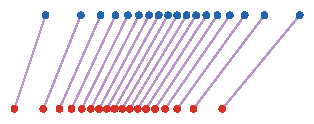
\includegraphics[width=.46\linewidth]{figures/matching-1d-convex-concave-costs/convex.pdf} &
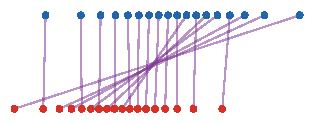
\includegraphics[width=.46\linewidth]{figures/matching-1d-convex-concave-costs/concave.pdf} \\[-.1em]
\small convex cost, $p=2$ &
\small concave cost, $p=1/2$ \\[.25em]
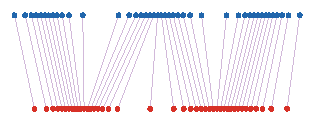
\includegraphics[width=.46\linewidth]{figures/matching-1d-convex-concave-costs/mixture-convex.pdf} &
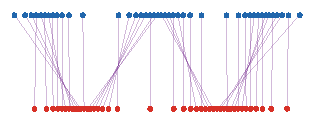
\includegraphics[width=.46\linewidth]{figures/matching-1d-convex-concave-costs/mixture-concave.pdf} \\[-.1em]
\small two-mode to three-mode, $p=2$ &
\small two-mode to three-mode, $p=1/2$
\end{tabular}
\caption{\emph{One-dimensional assignments for ordered source and target clouds with costs $c_p(x,y)=|x-y|^p$.} The top row uses single-Gaussian source and target clouds; the bottom row uses a denser two-component source and three-component target. For the convex quadratic cost, equal ranks are matched and the segments do not cross. For the concave cost, the optimum creates long crossing exchanges; the ordered line remains useful, but through the alternating-chain structure of concave transport rather than through monotone rearrangement.}
\index{monotone!rearrangement}% strictindex
\index{quadratic!cost}% strictindex
\label{fig:matching-1d-convex-concave-costs}
\end{figure}

\begin{figure}[H]
\centering
\begin{tabular}{@{}cc@{}}
\small two mixtures & \small one mode to three modes \\[-.15em]
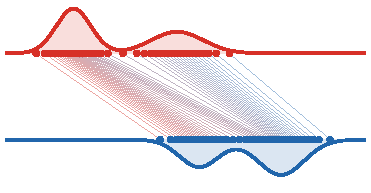
\includegraphics[width=.46\linewidth]{figures/matching-1d-quantile-assignment/quantile-assignment.pdf} &
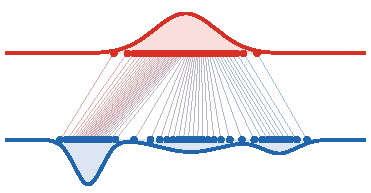
\includegraphics[width=.46\linewidth]{figures/matching-1d-quantile-assignment/central-to-three-modes.pdf}
\end{tabular}
\caption{\emph{One-dimensional optimal matching by quantile sorting.} The red and blue curves are smooth laws used to generate equal-weight empirical measures; the dots are inverse-CDF samples at common quantile levels. The monotone assignment connects equal ranks, both for two Gaussian mixtures and for the transport from one central Gaussian toward a three-mode target law.}
\index{Gaussian!mixture}% strictindex
\index{empirical!measure}% strictindex
\label{fig:matching-1d-quantile-assignment}
\end{figure}

\paragraph{Histogram equalization.}
Order preservation survives any strictly increasing change of coordinates. In particular, if $\phi:\RR\to\RR$ is strictly increasing and $h:\RR_+\to\RR$ is convex and nondecreasing, sorting solves the assignment problem for the cost $h(|\phi(x)-\phi(y)|)$ after applying $\phi$ to both clouds.

A typical application is grayscale histogram equalization. The empirical distribution of image luminances is transported to a prescribed target histogram, for instance a concentrated law or the histogram of a reference image. For equal-size samples with distinct ranks, monotone rearrangement gives the exact assignment. Repeated intensity values require a consistent tie-breaking or mass-splitting convention, but the same quantile construction remains the canonical one-dimensional solution. The operation matches distributions of intensities rather than spatial pixel locations.
\index{histogram}% strictindex
\index{transport!map}% strictindex
\index{monotone!rearrangement}% strictindex

\begin{figure}[H]
\centering
\begin{tabular}{@{}cccc@{}}
\small $t=0$ & \small $t=1/3$ & \small $t=2/3$ & \small $t=1$ \\[-.15em]

\includegraphics[width=.21\linewidth]{figures/monge-histogram-equalization/image-t000.pdf} &

\includegraphics[width=.21\linewidth]{figures/monge-histogram-equalization/image-t033.pdf} &

\includegraphics[width=.21\linewidth]{figures/monge-histogram-equalization/image-t067.pdf} &

\includegraphics[width=.21\linewidth]{figures/monge-histogram-equalization/image-t100.pdf} \\[-.1em]
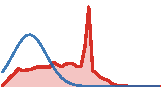
\includegraphics[width=.21\linewidth]{figures/monge-histogram-equalization/hist-t000.pdf} &
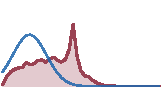
\includegraphics[width=.21\linewidth]{figures/monge-histogram-equalization/hist-t033.pdf} &

\includegraphics[width=.21\linewidth]{figures/monge-histogram-equalization/hist-t067.pdf} &

\includegraphics[width=.21\linewidth]{figures/monge-histogram-equalization/hist-t100.pdf}
\end{tabular}
\caption{\emph{Histogram equalization as one-dimensional Monge transport on pixel intensities.} The map is the monotone rearrangement $T=Q_\beta\circ F_\alpha$, using the cumulative and quantile functions defined later in Definition~\ref{def-cdf-quantile}; here $\beta$ is a truncated Gaussian concentrated near dark intensities. The images are interpolated pointwise by $I_t=(1-t)I+tT(I)$, and all histograms share the same vertical scale to make the displacement of intensity mass comparable across time.}
\index{cumulative function}% strictindex
\index{quantile!function}% strictindex
\index{monotone!rearrangement}% strictindex
\label{fig:monge-histogram-equalization}
\end{figure}

\paragraph{Flat directions for the linear cost.}
Strict convexity makes every optimizer increasing and, for distinct points, makes the optimizer unique. For a merely convex cost such as $|x-y|$, non-increasing optimal assignments can also exist. The next example shows that this is not a discretization artifact but a genuine flat direction of the linear cost.

\begin{example}[Discrete book-shifting and non-uniqueness for $\Wass_1$]\label{ex-book-shifting-w1}
\index{book-shifting}% strictindex
\index{Wasserstein!W1 non-uniqueness}% strictindex
	Fix $m\geq1$ and consider two equal-cardinality point clouds
	\[
		X=\{1,\ldots,2m\},
		\qquad
		Y=\{m+1,\ldots,3m\},
	\]
	with uniform weights. The monotone assignment sends $i$ to $i+m$ and has average cost $m$ for $c(x,y)=|x-y|$. It is not unique. The discrete book-shifting assignment
	\[
		T_{\rm book}(i)=
		\begin{cases}
			i+2m, & 1\leq i\leq m,\\
			i, & m<i\leq 2m,
		\end{cases}
	\]
	is also a bijection from $X$ to $Y$ and has the same average cost:
	\[
		\frac1{2m}\sum_{i=1}^{2m}|T_{\rm book}(i)-i|
		=
		\frac1{2m}\sum_{i=1}^{m}2m
		=m.
	\]
	Optimality follows from the lower bound
	\[
		\frac1{2m}\sum_{i=1}^{2m}|y_{\sigma(i)}-i|
		\geq
		\frac1{2m}\sum_{i=1}^{2m}(y_{\sigma(i)}-i)
		=m,
	\]
	which holds for every assignment because the target sum is fixed. The continuous Monge version of the same book-shifting phenomenon is given later in Example~\ref{ex-monge-book-shifting-w1}.
\index{book-shifting}% strictindex

	For $|x-y|^p$ with $p>1$, this degeneracy disappears: the monotone assignment has average cost $m^p$, whereas the book-shifting assignment has average cost $2^{p-1}m^p>m^p$. Strict convexity penalizes concentrating all displacement on half of the points.
\end{example}

\paragraph{Optimal transport on the circle.}\label{rem-circle-ot-cut}
\index{circle!transport}% strictindex

The sorting rule on the line has a periodic analogue. Identify the circle with $\mathbb S^1=\RR/\ZZ$, let
\[
	d_{\mathbb S^1}(x,y):=\min_{k\in\ZZ}|x-y+k|,
	\qquad
	c_p(x,y):=d_{\mathbb S^1}(x,y)^p,\qquad p>1.
\]
The only extra datum, compared with the line, is where one opens the circle. Once a cut has been chosen, the circle is unfolded into an interval and the one-dimensional monotone assignment can be used. In the discrete case, changing the cut is the same as applying a cyclic shift to one of the two circular orderings.
\index{cyclic!shift}% strictindex

\begin{proposition}[Discrete circle transport by a cut]\label{prop-circle-ot-cut}
\index{circle!transport}% strictindex
	Assume that the $2n$ points $x_1,\ldots,x_n,y_1,\ldots,y_n$ are pairwise distinct. Let $x_{(1)},\ldots,x_{(n)}$ and $y_{(1)},\ldots,y_{(n)}$ be fixed cyclic orderings, with indices understood modulo $n$. For $p>1$, every optimal assignment for the cost $c_p$ is a cyclic shift
	\[
		x_{(k)}\longmapsto y_{(k+s)},
		\qquad k\in\range{n},\quad s\in\{0,\ldots,n-1\}.
	\]
	Consequently, its cost is obtained by minimizing
	\[
		E_s
		\eqdef
		\frac1n\sum_{k=1}^n
		d_{\mathbb S^1}\!\left(x_{(k)},y_{(k+s)}\right)^p
	\]
	over the $n$ shifts. For each optimal assignment there is a cut $\theta\in\mathbb S^1\setminus(\{x_i\}_i\cup\{y_j\}_j)$, crossed by none of its shortest transport arcs, such that the lifted assignment on $(\theta,\theta+1)$ is the equal-rank matching on the line.
\index{monotone!matching}% strictindex
\end{proposition}

\begin{proof}
	Fix an optimal assignment $\sigma$ and let $\gamma_i$ be an open shortest arc from $x_i$ to $y_{\sigma(i)}$, with either orientation fixed in the antipodal case. The path-uncrossing lemma of Delon, Rabin and Gousseau states that if two arcs of an optimal assignment intersect, then they have the same orientation and neither is strictly contained in the other~\cite{DelonRabinGousseau2011Circle}. Its proof is a two-edge exchange: opposite orientations or strict containment would, by monotonicity and strict convexity of $r\mapsto r^p$, produce a strictly cheaper pairing of the four endpoints.

	Suppose that the arcs cover the circle. Since each $\gamma_i$ is open, every source point lies in another transport arc. Order the sources cyclically. The path-uncrossing lemma then propagates one common orientation: either $x_{(k+1)}\in\gamma_{(k)}$ for every $k$, or $x_{(k-1)}\in\gamma_{(k)}$ for every $k$. In the first case, define a new assignment by giving $x_{(k+1)}$ the target previously assigned to $x_{(k)}$; every transport arc becomes strictly shorter. The opposite orientation gives the analogous backward reassignment. Both contradict optimality. Hence some $\theta$ lies outside every transport arc.

	Cut the circle at such a $\theta$ and lift it to $(\theta,\theta+1)$. Every matched geodesic avoids the cut, so its circular length equals the ordinary distance between the corresponding lifts. Proposition~\ref{prop-matching-1d-monotone} now implies that the lifted matching preserves order. Returning to the circle, an order-preserving bijection between two cyclically ordered $n$-point sets is a cyclic shift. Minimizing over these $n$ shifts therefore recovers the optimum. This cut argument, including extensions to convex costs and nonuniform masses, is developed in~\cite{DelonRabinGousseau2011Circle,delon-circle}.
\index{circle!unfolded interval}% strictindex
\index{cyclic!shift}% strictindex
\end{proof}

\begin{alg}[Circle assignment by cutting]\label{alg:circle-cut-assignment}
\textbf{Input:} Equal-weight points $(x_i)_{i=1}^n$, $(y_j)_{j=1}^n$ on $\mathbb S^1$; cost $d_{\mathbb S^1}^p$.

\textbf{Output:} Optimal cyclic assignment and a compatible cut $\theta_{\rm cut}$.

\textbf{Let} $x_{(1)},\ldots,x_{(n)}$ and $y_{(1)},\ldots,y_{(n)}$ be the points sorted by increasing angle from a fixed origin.

\textbf{For} $s=0,\ldots,n-1$ \textbf{do}:
\begin{algblock}
\(E_s=n^{-1}\sum_{k=1}^n d_{\mathbb S^1}\!\left(x_{(k)},y_{(k+s)}\right)^p, \qquad y_{(k+n)}=y_{(k)}\).
\end{algblock}
\textbf{Set} $s^\star$ to the smallest minimizer of $(E_s)_{s=0}^{n-1}$.

\textbf{Construct} the shortest arcs from $x_{(k)}$ to $y_{(k+s^\star)}$.

\textbf{Choose} $\theta_{\rm cut}$ outside their union and outside all endpoints.

\textbf{Lift} every point to its representative in $(\theta_{\rm cut},\theta_{\rm cut}+1)$.

\textbf{Return} $x_{(k)}\mapsto y_{(k+s^\star)}$ and $\theta_{\rm cut}$.
\end{alg}

After sorting, this direct enumeration costs $O(n^2)$. The convex dependence of the circular transport cost on a continuous shift parameter leads to faster algorithms for general weighted histograms~\cite{delon-circle}.

\begin{figure}[H]
\centering
\begin{tabular}{cc}
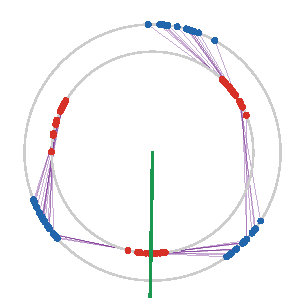
\includegraphics[width=.34\linewidth]{figures/monge-circle-cut-unfolding/circle.pdf} &
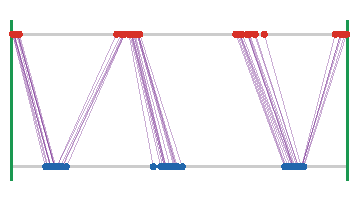
\includegraphics[width=.52\linewidth]{figures/monge-circle-cut-unfolding/unfolded.pdf} \\[-.1em]
\small circular problem &
\small unfolded interval
\index{circle!unfolded interval}% strictindex
\end{tabular}
\caption{\emph{Optimal transport on the circle by cutting and unfolding.} The red and blue atoms live on two copies of the circle; the denser point clouds make the cyclic ordering visible. Purple segments show the optimal matching and the green radius marks the chosen cut. Once the circle is opened at this angle, the same matching appears as a monotone one-dimensional assignment on the interval, with the two green endpoints identified.}
\index{circle!transport}% strictindex
\label{fig:monge-circle-cut-unfolding}
\end{figure}

\begin{figure}[H]
\centering
\setlength{\tabcolsep}{1.5pt}
\begin{tabular}{@{}cccc@{}}
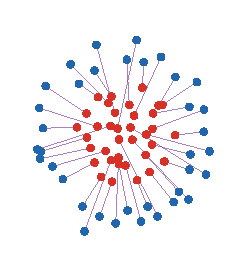
\includegraphics[width=.232\linewidth]{figures/matching-2d-cost-exponent/p0p5.pdf} &

\includegraphics[width=.232\linewidth]{figures/matching-2d-cost-exponent/p1.pdf} &

\includegraphics[width=.232\linewidth]{figures/matching-2d-cost-exponent/p2.pdf} &
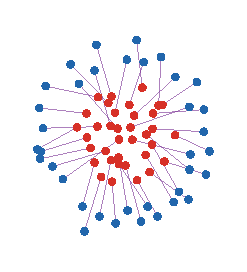
\includegraphics[width=.232\linewidth]{figures/matching-2d-cost-exponent/p6.pdf} \\[-.1em]
\small $c(x,y)=\norm{x-y}^{1/2}$ &
\small $c(x,y)=\norm{x-y}$ &
\small $c(x,y)=\norm{x-y}^2$ &
\small $c(x,y)=\norm{x-y}^6$
\end{tabular}
\caption{\emph{Optimal assignments between the same two point clouds for four powers of the Euclidean distance.} The source atoms are semi-regular samples in a central disk, while the target atoms are semi-regular samples on a thin annulus; this canonical geometry is reused in later coupling and regularization figures. The feasible set is unchanged, but changing $p$ changes the global organization of the permutation: the concave case $p=1/2$ penalizes long edges only sublinearly and therefore permits longer exchanges, whereas larger powers increasingly suppress the longest edges.}
\label{fig:matching-2d-cost-exponent}
\end{figure}

\paragraph{Rational weights.}
\index{rational weights}% strictindex

The strict assignment model is also tied to equal cardinalities and equal weights. As soon as the target resolution changes or the weights are not uniform, a permutation no longer describes the feasible transports. One instead needs a nonnegative transport matrix with prescribed row and column sums, as illustrated in Figure~\ref{fig:matching-resolution-and-weights}; this is the finite-dimensional Kantorovich relaxation developed in Chapter~\ref{sec-kantorovich}.
\index{nonnegative transport matrix}% strictindex
\index{Kantorovich!relaxation}% strictindex

\begin{figure}[H]
\centering
\begin{tabular}{ccc}

\includegraphics[width=.30\linewidth]{figures/matching-resolution-and-weights/balanced.pdf} &
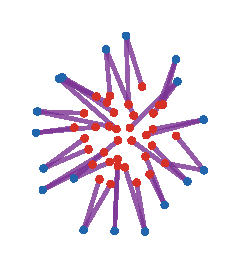
\includegraphics[width=.30\linewidth]{figures/matching-resolution-and-weights/rectangular.pdf} &
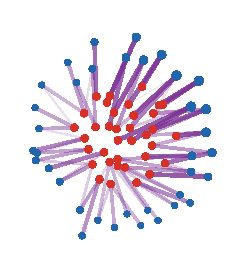
\includegraphics[width=.30\linewidth]{figures/matching-resolution-and-weights/weighted.pdf} \\[-.1em]
\small $n=m$ &
\small $m<n$ &
\small $n=m$ but $\b_j\neq 1/n$
\end{tabular}
\caption{\emph{From assignments to transport plans, using the same disk-to-annulus geometry as Figure~\ref{fig:matching-2d-cost-exponent}.} In the balanced equal-weight case, each source atom is matched to one target atom. With a target cloud that has half as many atoms, or with strongly nonuniform target weights, the coupling matrix can merge or split mass; segment thickness and opacity encode its nonzero entries, and blue marker areas encode the prescribed target masses.}
\index{plan!transport}% strictindex
\label{fig:matching-resolution-and-weights}
\end{figure}

\begin{proposition}[Rational weights as duplicated uniform matching]\label{prop-rational-weights-duplicated-matching}
\index{rational weights}% strictindex
\index{matching!uniform}% strictindex
	Let
	\[
		\alpha=\sum_{i=1}^n \frac{k_i}{N}\delta_{x_i},
		\qquad
		\beta=\sum_{j=1}^m \frac{\ell_j}{N}\delta_{y_j},
		\qquad
		\sum_i k_i=\sum_j\ell_j=N,
	\]
	with positive integers $k_i,\ell_j$. Replace each $x_i$ by $k_i$ identical copies and each $y_j$ by $\ell_j$ identical copies, producing two uniform $N$-point clouds. Then the duplicated assignment problem and the discrete Kantorovich problem between $\alpha$ and $\beta$ have the same optimal value. Moreover, there exists an optimal coupling of the form
	\[
		P_{ij}=\frac{n_{ij}}{N},
		\qquad
		n_{ij}\in\NN,
		\qquad
		\sum_j n_{ij}=k_i,
		\quad
		\sum_i n_{ij}=\ell_j,
	\]
	and couplings whose scaled entries $NP_{ij}$ are integral are exactly the collapsed assignments between duplicated clouds. Fractional optimal couplings may nevertheless coexist when the optimum is degenerate.
\index{Kantorovich!problem}% strictindex
\index{optimal coupling}% strictindex
\index{assignment problem}% strictindex
\end{proposition}
\begin{proof}
	Any assignment between the duplicated source and target clouds defines integers $n_{ij}$ counting how many copied particles of type $x_i$ are matched to copied particles of type $y_j$. These counts satisfy $\sum_j n_{ij}=k_i$ and $\sum_i n_{ij}=\ell_j$, and the associated coupling $P_{ij}=n_{ij}/N$ has marginals $k_i/N$ and $\ell_j/N$. The assignment cost is
\index{cost!assignment}% strictindex
	\[
		\frac1N\sum_{i,j} n_{ij}c(x_i,y_j)
		=
		\sum_{i,j}P_{ij}c(x_i,y_j).
	\]
	Conversely, any nonnegative integer count matrix with those row and column sums can be realized by allocating the $k_i$ copies of each $x_i$ among the target copies according to $(n_{ij})_j$. It remains to show that restricting to integral counts does not increase the optimum. Scale a feasible coupling by $N$ and write $Q=NP$. The constraints on $Q$ have integer right-hand sides $(k_1,\ldots,k_n,\ell_1,\ldots,\ell_m)$. After multiplying the target rows by $-1$, their coefficient matrix is the oriented node-edge incidence matrix of a bipartite graph and is therefore totally unimodular. Every vertex of this transportation polytope is integral. Since a linear objective attains its minimum at a vertex, an integral optimal $Q$ exists, proving equality of the two optimal values. The argument establishes existence, not integrality of every optimizer; convex combinations of distinct integral optima give fractional optima.
\index{total unimodularity}% strictindex
\index{transportation polytope}% strictindex
\index{assignment problem}% strictindex
\end{proof}

This network-flow integrality mechanism is the rational-weight counterpart of the Birkhoff--von Neumann theorem proved later in Theorem~\ref{thm-birkhoff-von-neumann}: in both cases, a linear transport relaxation has an optimizer represented by integer edge flows after scaling. The equal-unit-margin case specializes these flows to permutation matrices, whereas a degenerate optimal face may also contain fractional couplings.

\begin{figure}[H]
\centering
\begin{tabular}{ccc}
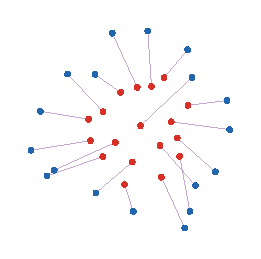
\includegraphics[width=.30\linewidth]{figures/matching-rational-duplication/uniform.pdf} &
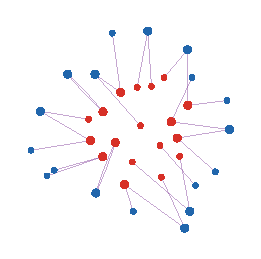
\includegraphics[width=.30\linewidth]{figures/matching-rational-duplication/binary.pdf} &
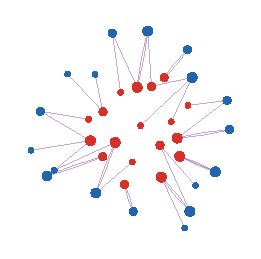
\includegraphics[width=.30\linewidth]{figures/matching-rational-duplication/ternary.pdf} \\[-.1em]
\small $k_i=\ell_j=1$ &
\small $k_i,\ell_j\in\{1,2\}$ &
\small $k_i,\ell_j\in\{1,2,3\}$
\end{tabular}
\caption{\emph{Rational weights as duplicated uniform matchings, using the same disk-to-annulus geometry as Figure~\ref{fig:matching-resolution-and-weights} with fewer displayed atoms.} The red and blue locations are kept fixed, while disk areas encode the integer multiplicities $k_i$ and $\ell_j$. Solving the assignment problem after duplicating particles produces several collapsed segments attached to high-multiplicity atoms; this is the integer count matrix of Proposition~\ref{prop-rational-weights-duplicated-matching}.}
\index{integer multiplicity}% strictindex
\index{assignment problem}% strictindex
\index{rational weights}% strictindex
\index{matching!uniform}% strictindex
\label{fig:matching-rational-duplication}
\end{figure}

\paragraph{Two-dimensional geometry.}

Sorting no longer orders a planar cloud, but a simple local exchange still rules out proper crossings for the Euclidean-distance cost. This observation, already present in Monge's geometric reasoning, is necessary but far from sufficient for computing an optimum.

\begin{proposition}[No proper crossings in Euclidean-distance matchings]\label{prop-planar-no-proper-crossing}
\index{matching!non-crossing}% strictindex
	Let $x_1,\ldots,x_n,y_1,\ldots,y_n\in\RR^2$ and let $c(x,y)=\norm{x-y}$. If $\sigma$ is optimal, then two matched segments cannot cross properly: their relative interiors cannot meet at a point where their supporting lines are distinct.
\end{proposition}

\begin{proof}
	Suppose that $[x_i,y_{\sigma(i)}]$ and $[x_j,y_{\sigma(j)}]$ cross properly at $z$. The triangle inequality along the two reconnected paths gives
\index{triangle inequality}% strictindex
	\[
		\norm{x_i-y_{\sigma(j)}}
		\leq
		\norm{x_i-z}+\norm{z-y_{\sigma(j)}},
	\]
	and
	\[
		\norm{x_j-y_{\sigma(i)}}
		\leq
		\norm{x_j-z}+\norm{z-y_{\sigma(i)}}.
	\]
	The sum of the two right-hand sides is exactly the cost of the two original segments. At least one inequality is strict because a proper crossing is non-collinear. Swapping $\sigma(i)$ and $\sigma(j)$ therefore strictly decreases the assignment cost, contradicting optimality. Collinear overlaps are excluded from the statement precisely because the exchange can then have equal cost.
\end{proof}

This property alone is, however, not enough to lead to an efficient algorithm. Non-crossing is only a necessary local test, not a compact certificate of optimality. For instance, if $n$ sources and $n$ targets are placed alternately on the boundary of a convex polygon, the number of non-crossing perfect matchings is the Catalan number
\index{matching!perfect}% strictindex
\index{Catalan number}% strictindex
\[
	C_n=\frac{1}{n+1}\binom{2n}{n}\sim \frac{4^n}{\sqrt{\pi}n^{3/2}}.
\]

\begin{rem}[Catalan count of alternating non-crossing matchings]
\index{matching!non-crossing}% strictindex
	The count follows from the standard Catalan recurrence. Fix one red vertex $r$. In a non-crossing perfect matching, if $r$ is matched to a blue vertex $b$, the chord $[r,b]$ splits the polygon into two smaller polygons. Since the boundary colors alternate, each side contains the same number of red and blue vertices. If one side contains $k$ red and $k$ blue vertices, the other contains $n-1-k$ red and $n-1-k$ blue vertices. Non-crossing matchings on the two sides are independent, because no segment can cross the chord $[r,b]$. Thus, denoting by $M_n$ the number of such matchings, one has
\index{matching!perfect}% strictindex
	\[
		M_0=1,
		\qquad
		M_n=\sum_{k=0}^{n-1} M_k M_{n-1-k}.
	\]
	This recurrence characterizes the Catalan numbers, hence $M_n=C_n$.
\index{Catalan number}% strictindex
\end{rem}

Thus even after forbidding proper crossings, exhaustive search remains exponential. The two-segment swap explains why a transverse crossing cannot be optimal, but it does not select among the exponentially many planar matchings that survive this local test.


%%%%%%%%%%%%%%%%%%%%%%%%%%%%%%%%%%%%%%%%%%%%%%%%%%%%%%%%%%%%%%%%%%%%%%%%%%%
\section{Matching Algorithms}
\index{matching!algorithm}% strictindex

This section briefly locates matching within classical combinatorial optimization. Its main point is that efficient algorithms exist, but their cleanest analysis is obtained only after introducing the linear-programming viewpoint.

\paragraph{Classical assignment methods.}
\index{assignment problem}% strictindex
Efficient algorithms avoid enumerating $n!$ permutations. The most familiar classical examples are the Hungarian method and auction algorithms~\cite{Kuhn1955,bertsekas1981new,bertsekas1992auction,Burkard09}. Auction algorithms attach prices to targets: an unmatched source bids for the target of smallest reduced cost, equivalently largest reduced profit, and raises that target's price. The process terminates once $\epsilon$-complementary slackness holds. For integer costs, this condition places the unnormalized total cost within $n\epsilon$ of optimum. If $\epsilon<1/n$, the resulting integer assignment cost is less than one above the integer optimum and must therefore equal it~\cite{bertsekas1992auction}. Section~\ref{sec-auction-dual-ascent} revisits the method after Kantorovich duality and explains why it is a dual price algorithm, parallel in spirit to Sinkhorn scaling.
\index{Sinkhorn!scaling}% strictindex
\index{Hungarian primal-dual method}% strictindex
\index{complementary slackness}% strictindex
\index{Kantorovich!duality}% strictindex
\index{auction algorithm}% strictindex
\index{assignment problem}% strictindex

\paragraph{Hungarian primal-dual method.}
\index{Hungarian primal-dual method}% strictindex
\index{assignment problem}% strictindex

The Hungarian method is best understood as a certificate-building algorithm for the assignment linear program. Since the factor $1/n$ in~\eqref{eq-optimal-assignment} does not affect the optimizer, we work with the unnormalized total cost. The method maintains a partial matching $M$ and dual labels $(u_i,v_j)$ satisfying
\index{partial matching}% strictindex
\index{dual!price}% strictindex
\[
	 u_i+v_j\leq \C_{i,j}\qquad\forall i,j.
\]
The equality graph $E(u,v)=\{(i,j):u_i+v_j=\C_{i,j}\}$ contains the zero-reduced-cost edges. For a source set $S$, write $N_E(S)=\{j:\exists i\in S,\ (i,j)\in E(u,v)\}$ for its target neighborhood. The algorithm only augments $M$ along alternating paths of equality edges. Starting from an unmatched source, it grows an alternating tree with source set $S$ and target set $T$. If the tree reaches an unmatched target, the matching is augmented along the path. If $N_E(S)\setminus T$ is empty, the dual labels are shifted by the smallest slack
\index{alternating!tree}% strictindex
\index{graph!equality}% strictindex
\index{cost!reduced}% strictindex
\index{slack variable}% strictindex
\[
	\delta=\min_{i\in S,\ j\notin T}\bigl(\C_{i,j}-u_i-v_j\bigr),
	\qquad
	u_i\leftarrow u_i+\delta\ (i\in S),\qquad
	v_j\leftarrow v_j-\delta\ (j\in T).
\]
This update preserves all inequalities $u_i+v_j\leq \C_{i,j}$, keeps the current alternating tree tight, and creates at least one new equality edge leaving $S$. Maintaining these slacks incrementally gives the standard $O(n^3)$ implementation for an $n\times n$ assignment problem.
\index{assignment problem}% strictindex
\index{alternating!tree}% strictindex
Algorithm~\ref{alg:hungarian-primal-dual} summarizes the primal-dual loop. Figure~\ref{fig:matching-hungarian-progression} displays actual iterates by showing only the evolving partial assignment: unmatched rows are shown as flat rows to keep a fixed matrix format, and matched rows are shown as one-hot rows.
\index{Hungarian primal-dual method}% strictindex

\begin{alg}[Hungarian primal-dual augmentation]\label{alg:hungarian-primal-dual}
\textbf{Input:} Square cost matrix $\C\in\RR^{n\times n}$.

\textbf{Output:} Minimum-cost perfect matching $M$.

\textbf{Initialize:} Set $u_i=\min_j \C_{ij}$ and $v_j=0$.

\textbf{Set} $M=\emptyset$.

\textbf{While} $M$ is not perfect \textbf{do}:
\begin{algblock}

\textbf{Build} equality graph:
\(E(u,v)=\{(i,j):u_i+v_j=\C_{i,j}\}\).

\textbf{Set} root $i_0=\min\{i:\ i\text{ is unmatched in }M\}$.

\textbf{Set} reached sets $S=\{i_0\}$ and $T=\emptyset$; clear parent pointers.

\textbf{While} $T$ contains no unmatched target \textbf{do}:
\begin{algblock}

\textbf{If} $N_E(S)\setminus T=\emptyset$ \textbf{then}:
\begin{algblock}

\textbf{Compute} $\delta=\min_{i\in S,\ j\notin T}\bigl(\C_{i,j}-u_i-v_j\bigr)$.

\textbf{Update} $u_i\leftarrow u_i+\delta$ for $i\in S$ and $v_j\leftarrow v_j-\delta$ for $j\in T$.

\textbf{Refresh} equality graph $E(u,v)$.

\end{algblock}
\textbf{Set} $J=N_E(S)\setminus T$.

\textbf{For} each $j\in J$ in increasing order \textbf{do}:
\begin{algblock}

\textbf{Add} $j$ to $T$ and set parent row $p(j)=\min\{i\in S:(i,j)\in E(u,v)\}$.

\textbf{If} $j$ is matched to $i'$ in $M$ \textbf{then set} \(S\leftarrow S\cup\{i'\}\) and \(q(i')=j\).

\end{algblock}
\end{algblock}
\textbf{Set} $j_0=\min\{j\in T:\ j\text{ is unmatched in }M\}$.

\textbf{Set} $j=j_0$.

\textbf{While} $j$ is defined \textbf{do}:
\begin{algblock}

\textbf{Set} $i=p(j)$.

\textbf{Set} $j_{\rm old}=q(i)$.

\textbf{If} $j_{\rm old}$ is defined \textbf{then set} \(M\leftarrow M\setminus\{(i,j_{\rm old})\}\).

\textbf{Set} $M\leftarrow M\cup\{(i,j)\}$.

\textbf{Set} $j=j_{\rm old}$.
\end{algblock}
\end{algblock}
\algreturnskip
\textbf{Return} $M$.
\end{alg}

\begin{figure}[H]
\centering
\setlength{\tabcolsep}{2pt}
\begin{tabular}{ccccc}

\includegraphics[width=.18\linewidth]{figures/matching-hungarian-progression/stage-0.pdf} &

\includegraphics[width=.18\linewidth]{figures/matching-hungarian-progression/stage-1.pdf} &

\includegraphics[width=.18\linewidth]{figures/matching-hungarian-progression/stage-2.pdf} &

\includegraphics[width=.18\linewidth]{figures/matching-hungarian-progression/stage-3.pdf} &

\includegraphics[width=.18\linewidth]{figures/matching-hungarian-progression/stage-4.pdf} \\[-.1em]
\small initial &
\small 2 aug. &
\small 4 aug. &
\small 6 aug. &
\small final
\end{tabular}
\caption{\emph{Matrix view of actual Hungarian primal-dual iterates on a diagonally dominant ordered one-dimensional squared-distance assignment.} Each panel records the current partial assignment state: unassigned rows are kept flat, while assigned rows are one-hot. The snapshots are taken at initialization and after two, four, six and eight augmentations; for this pedagogical instance the partial assignments grow along the diagonal, and the final matrix is the identity assignment certified by complementary slackness.}
\index{complementary slackness}% strictindex
\label{fig:matching-hungarian-progression}
\end{figure}

\begin{prop}[Correctness and complexity of the Hungarian primal-dual method]\label{prop-hungarian-correct}
\index{Hungarian primal-dual method}% strictindex
	Assume the Hungarian method terminates with a perfect matching $\sigma$ contained in the equality graph
\index{matching!perfect}% strictindex
\index{graph!equality}% strictindex
	\[
		E(u,v)=\enscond{(i,j)}{u_i+v_j=\C_{i,j}},
	\]
	where $(u,v)$ is dual feasible, i.e. $u_i+v_j\leq \C_{i,j}$ for all $(i,j)$. Then $\sigma$ is an optimal assignment. Moreover, the usual Hungarian updates terminate after finitely many augmentations.
	With maintained slacks, the method uses $O(n^3)$ arithmetic operations.
\end{prop}

\begin{proof}
	For any permutation $\tau$, dual feasibility gives
	\[
		\sum_i \C_{i,\tau(i)} \geq \sum_i (u_i+v_{\tau(i)})
		= \sum_i u_i+\sum_j v_j.
	\]
	This is the weak duality lower bound. If $\sigma$ is contained in the equality graph, then
\index{duality!weak}% strictindex
\index{graph!equality}% strictindex
	\[
		\sum_i \C_{i,\sigma(i)}
		= \sum_i u_i+\sum_j v_j,
	\]
	so the primal cost of $\sigma$ reaches the dual lower bound and is optimal.

	It remains to justify finite termination and the complexity bound. At each successful augmentation, the matching cardinality increases by one, so there are exactly $n$ augmentation phases. During one phase, the algorithm grows an alternating tree in the equality graph. Before reaching a free target, the tree invariant is $|S|=|T|+1$, so $T$ cannot contain every target. If $N_E(S)\setminus T$ is empty, every slack from $S$ to $T^c$ is positive and the minimum defining $\delta$ exists. For edges in $S\times T$, adding $\delta$ to source labels and subtracting it from target labels preserves tightness. For edges in $S\times T^c$, the definition of $\delta$ preserves feasibility and makes at least one new edge tight; edges in $S^c\times T$ become looser, and all remaining inequalities are unchanged. Thus the reachable sets strictly grow after every dual update and can grow at most $n$ times in one phase. If the slacks $\min_{i\in S}(\C_{i,j}-u_i-v_j)$ are maintained when a source enters $S$, each tree expansion costs $O(n)$. A phase costs $O(n^2)$ and the $n$ phases cost $O(n^3)$. Hence the method reaches a perfect optimal matching.
\index{tightness}% strictindex
\index{alternating!tree}% strictindex
\index{graph!augmenting path}% strictindex
\index{graph!equality}% strictindex
\end{proof}

The chapter has thus exposed two complementary routes to finite matching: geometric structure can reduce the problem to sorting, while primal-dual labels provide a global certificate for an arbitrary cost matrix. The next chapter passes from finite permutations to transport maps between general measures.
